\documentclass{beamer}
\usetheme{chlenski}
\usepackage[utf8]{inputenc}
\usepackage{graphicx}
\usepackage{outlines}
\usepackage[nodisplayskipstretch]{setspace}

\title{Intro to Microbial Genomics}
\subtitle{BIOL BC3308, Lecture 3}
\author{Philippe Chlenski}
\date{January 31, 2023}

\renewcommand{\c}[1]{\begin{center}#1\end{center}}
\newcommand{\blu}[1]{\textcolor{blue}{\textbf{#1}}}
\newcommand{\red}[1]{\textcolor{red}{\textbf{#1}}}
\newcommand{\yel}[1]{\textcolor{yellow}{\textbf{#1}}}
\newcommand{\grn}[1]{\textcolor{dark-green}{\textbf{#1}}}
\newcommand{\prp}[1]{\textcolor{purple}{\textbf{#1}}}
\newcommand{\gr}[2][.95]{\c{\includegraphics[width=#1\textwidth]{#2}}}

% \setbeameroption{show notes}

\begin{document}

\begin{frame}[plain]
\titlepage
\end{frame}

\begin{frame}{Outline}
\tableofcontents
\end{frame}

\section{Background and motivation}

\begin{frame}{Overview}
\begin{outline}
\1[] \blu{Questions:}
    \2 Why do we compare sequences?
    \2 What is a sequence alignment and how do we make one?
\1[] \blu{Theory:}
    \2 Dot matrices
    \2 Global alignment algorithm
    \2 Local alignment algorithm
\1[] \blu{Practice:}
    \2 Creating scoring and traceback matrices
    \2 Using Biopython to generate sequence alignments
    \2 Implementing BLAST
\end{outline}
\end{frame}

\begin{frame}{Why compare sequences?}
To obtain functional or mechanistic insight about a sequence by inference from another potentially better characterized sequence\\
\bigskip
To find whether two (or more) genes or proteins are evolutionarily related\\
\bigskip
To find structurally or functionally similar regions within sequences (e.g., catalytic sites, binding sites, etc.)\\
\bigskip
Any others you can think of?
\end{frame}

\begin{frame}{Practical applications}
\begin{outline}
    \1[] \blu{Similarity searching of databases}
        \2 Say we sequenced a gene but don’t know the function. We can search GenBank for a similar gene and use that gene’s annotation to infer the function of ours.
    \1[] \blu{Assembly of sequence reads}
        \2 Sequence comparisons can allow us to combine short reads into a longer construct such as a genomic sequence or contig.
    \1[] \blu{Mapping sequencing reads to a known genome}
        \2 Ex: Known as “re-sequencing”, looking for differences from a reference genome (SNPs, indels, etc.)
        \2 Pretty much all of next-gen sequencing analysis.
\end{outline}
\end{frame}

\begin{frame}{Alignment intuition}
\blu{Basic concept:} Display one sequence above another with spaces (gaps) inserted into both to reveal similarity of nucleotides or amino acids:\\
\bigskip \noindent
\texttt{\blu{Seq1}: C A T T C A C\\
\hspace{3em} \\
\blu{Seq2}: C T C G C A G C
}
\end{frame}

\begin{frame}{Alignment intuition, cont}
\blu{Basic concept:} Display one sequence above another with spaces (gaps) inserted into both to reveal similarity of nucleotides or amino acids:\\
\bigskip \noindent
\texttt{\blu{Seq1}: \grn{C} \red{A T T} \grn{C A} \red{C}\\
\hspace{3em} \grn{|} \hspace{2.5em} \grn{| |} \\
\blu{Seq2}: \grn{C} \red{T C G} \grn{C A} \red{G C}
}\\
\bigskip
\begin{columns}
    \begin{column}{0.5\textwidth}
        Two types of character correspondence:\\
        \begin{outline}
            \1 \grn{Match}
            \1 \red{Substitution}
        \end{outline}
    \end{column}
    \begin{column}{0.5\textwidth}
    \hspace{1em}
    \end{column}
\end{columns}
\end{frame}

\begin{frame}{Alignment intuition, cont}
\blu{Basic concept:} Display one sequence above another with spaces (gaps) inserted into both to reveal similarity of nucleotides or amino acids:\\
\bigskip \noindent
\texttt{\blu{Seq1}: \grn{C} \yel{A} \grn{T} \prp{-} \red{T} \grn{C A} \prp{-} \grn{C}\\
\grn{\hspace{3em} |\hspace{1.5em}|\hspace{2.5em}| |\hspace{1.5em}|}\\
\blu{Seq2}: \grn{C} \yel{-} \grn{T} \prp{C} \red{G} \grn{C A} \prp{G} \grn{C}
}\\
\bigskip
\begin{columns}
    \begin{column}{0.5\textwidth}
        Two types of character correspondence:\\
        \begin{outline}
            \1 \grn{Match}
            \1 \red{Substitution}
        \end{outline}
    \end{column}
    \begin{column}{0.5\textwidth}
    Two types of sequence gap (AKA indel):
    \begin{outline}
        \1 \yel{Deletion}
        \1 \prp{Insertion}
    \end{outline}
    \end{column}
\end{columns}
\end{frame}

\begin{frame}{Sequence changes during evolution}
Three major mutations can occur in a genetic sequence over the course of evolution:
\begin{enumerate}
    \item Substitutions
    \item Deletions
    \item Insertions
\end{enumerate}
\gr{l3_figs/s8_tree.png}
\end{frame}

\begin{frame}{Sequence changes during evolution, cont}
Three major mutations can occur in a genetic sequence over the course of evolution:
\begin{enumerate}
    \item \red{Substitutions}
    \item Deletions
    \item Insertions
\end{enumerate}
\gr{l3_figs/s9_tree.png}
\end{frame}

\begin{frame}{Sequence changes during evolution, cont}
Three major mutations can occur in a genetic sequence over the course of evolution:
\begin{enumerate}
    \item Substitutions
    \item Deletions
    \item Insertions
\end{enumerate}
\gr{l3_figs/s10_tree.png}
\end{frame}

\begin{frame}{Sequence changes during evolution, cont}
Three major mutations can occur in a genetic sequence over the course of evolution:
\begin{enumerate}
    \item Substitutions
    \item \yel{Deletions}
    \item Insertions
\end{enumerate}
\gr{l3_figs/s11_tree.png}
\end{frame}

\begin{frame}{Sequence changes during evolution, cont}
Three major mutations can occur in a genetic sequence over the course of evolution:
\begin{enumerate}
    \item Substitutions
    \item Deletions
    \item \prp{Insertions}
\end{enumerate}
\gr{l3_figs/s12_tree.png}
\end{frame}

\begin{frame}{Sequence changes during evolution, cont}
Three major mutations can occur in a genetic sequence over the course of evolution:
\begin{enumerate}
    \item \red{Substitutions}
    \item Deletions
    \item Insertions
\end{enumerate}
\gr{l3_figs/s13_tree.png}
\end{frame}

\section{Alignment}

\begin{frame}{Alignment view}
Alignments are great tools to visualize sequence similarity and evolutionary changes in homologous sequences:
\begin{outline}
\1 \blu{Mismatches} represent mutations/substitutions
\2 \blu{Gaps} represent insertions and deletions (indels)
\gr{l3_figs/s14_alignment.png}
\end{outline}
\end{frame}

\begin{frame}{Alternative alignments}
Finding the correct alignment can be difficult if we don't know the evolutionary history of our sequences.\\
\bigskip
Which of the following alignments is best?
\gr{l3_figs/s15_alt_alignments.png}
\end{frame}

\begin{frame}{Alternative alignments, cont}
Finding the correct alignment can be difficult if we don't know the evolutionary history of our sequences.\\
\bigskip
Which of the following alignments is best?
\gr{l3_figs/s16_alt_alignments.png}
\end{frame}

\begin{frame}{Optimal alignments}
We may prefer \blu{parsimonious alignments}: explaining the differences between two sequences using the least mutations.\\
\bigskip
Here is one example of a scoring scheme: \gr{l3_figs/s17_alt_alignments.png}
\tiny \centering{Q: Can you spot a second optimal alignment in \#2?}
\end{frame}

\begin{frame}{Optimal alignments, cont}
We may prefer \blu{parsimonious alignments}: explaining the differences between two sequences using the least mutations.\\
\bigskip
Here is one example of a scoring scheme: \gr{l3_figs/s18_alt_alignments.png}\tiny \centering{Q: Can you spot a second optimal alignment in \#2?}
\end{frame}

\begin{frame}{Dot plots: a simple graphical approach to alignment}
1. Place one sequence along the vertical axis and a second sequence along the horizontal axis to form a matrix:
\gr[.5]{l3_figs/s19_matrix.png}
\end{frame}

\begin{frame}{Dot plots, cont}
2. Place dots wherever the horizontal and vertical characters match:
\gr[.5]{l3_figs/s20_matrix.png}
\end{frame}

\begin{frame}{Dot plots, cont}
3. Interpretation: diagonal runs of dots indicate matched segments of sequence.
\gr[0.5]{l3_figs/s21_matrix.png}
\centering{\tiny Question: what would a dot plot of two identical sequences look like?}
\end{frame}

\begin{frame}{Dot plots, cont}
Dot plots for long sequences can be noisy!
\gr[0.5]{l3_figs/s23_dotplot.png}
\end{frame}

\begin{frame}{Dot plot window size and match stringency}
Solution: use a window and a threshold
\begin{outline}
\1 Compare character-by-character inside a window
\1 Require a certain fraction of matches within each window (stringency)
\1 User input: window size and stringency parameters 
\end{outline}
\gr[0.5]{l3_figs/s24_windows.png}
\end{frame}

\begin{frame}{Dot plot window size and match stringency, cont}
Solution: use a window and a threshold
\begin{outline}
\1 Compare character-by-character inside a window
\1 Require a certain fraction of matches within each window (stringency)
\1 User input: window size and stringency parameters 
\end{outline}
\gr[0.5]{l3_figs/s25_windows.png}
\end{frame}

\begin{frame}{What does changing window size do?}
\gr{l3_figs/s27_sizes.png}
\begin{outline}
    \2 Requiring 5 bases to perfect match is a heuristic – only look at regions that have a certain degree of identity
    \2 Do you expect evolutionarily related sequences to have more word matches (matches in a row over a certain length) than random unrelated sequences?
    \2 Only diagonals can be followed; downwards or rightward paths represent insertion or deletions
\end{outline}
\end{frame}

\begin{frame}{Uses for dot plots}
\begin{outline}
\1 Visually assessing the similarity of two protein or nucleic acid sequences
\1 Finding local repeat sequences within a larger sequences by comparing a sequence to itself
    \2 Question: what would a repeat look like on a dot plot?
\end{outline}
\end{frame}

\section{Dynamic programming}

\begin{frame}{Dynamic programming algorithms}
The dynamic programming algorithm is an extension of the dot plot approach:
\begin{outline}
\1 One sequence is placed down the size of a grid and the second across the top
\1 Instead of placing dots, we compute a score for each position
\1 The optimal alignment corresponds to finding the path through the grid with the best possible score
\end{outline}
\gr{l3_figs/s29_dynamic.png}
\end{frame}

\begin{frame}{Needleman-Wunsch}
The Needleman-Wunsch approach to global alignment is an algorithm with three basic steps:\\
\bigskip
1. \blu{Set up a 2D grid} (or alignment matrix). Add gaps in the first row and column.
\begin{columns}
\begin{column}{0.5\textwidth}
    \gr{l3_figs/s30_nw.png}
\end{column}
\begin{column}{0.5\textwidth}
\hspace{1em}
\end{column}
\end{columns}
\end{frame}

\begin{frame}{Needleman-Wunsch, cont}
The Needleman-Wunsch approach to global alignment is an algorithm with three basic steps:\\
\bigskip
2. \blu{Score the matrix}. Start by filling the first rows and columns with indels, accumulating gap penalties.
\begin{columns}
\begin{column}{0.5\textwidth}
    \gr{l3_figs/s31_nw.png}
\end{column}
\begin{column}{0.5\textwidth}
\tiny
\red{Scoring scheme:}
\begin{outline}
\1 Match: +1
\1 Mismatch: -1
\1 Gap: -2
\end{outline}
\bigskip
\red{First column alignment:}\\
\noindent
\texttt{%
\blu{Seq1}: D P M E \ldots\\
\blu{Seq2}: - - - - \ldots
}
\end{column}
\end{columns}
\end{frame}

\begin{frame}{Needleman-Wunsch, cont}
The Needleman-Wunsch approach to global alignment is an algorithm with three basic steps:\\
\bigskip
2. \blu{Score the matrix}. Then, go the empty corner top-left corner cell. Which of its three neighbors gives us the best score?
\begin{columns}
\begin{column}{0.5\textwidth}
    \gr{l3_figs/s33_nw.png}
\end{column}
\begin{column}{0.5\textwidth}
\tiny
\[
S_{(i,j)} = \max \begin{cases}
    S_{(i-1,j-1)} + \text{(mis)match} &\textcolor{red}{\searrow}\\
    S_{(i-1,j)} + \text{gap penalty} &\textcolor{red}{\downarrow}\\
    S_{(i,j-1)} + \text{gap penalty} &\textcolor{red}{\rightarrow}
\end{cases}
\]
\centering{
    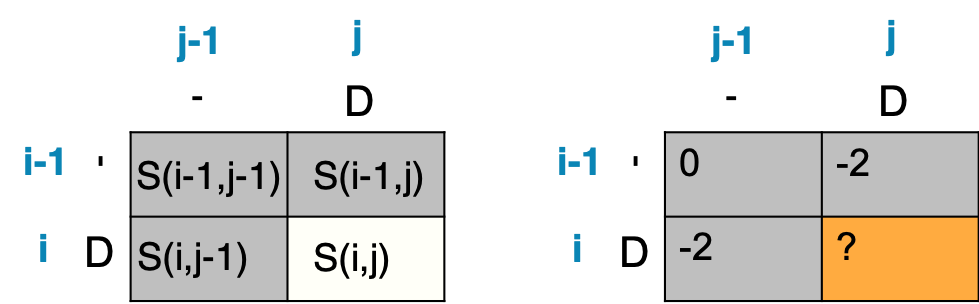
\includegraphics[width=0.7\textwidth]{l3_figs/s33_coords.png}
}
\end{column}
\end{columns}
\end{frame}

\begin{frame}{Needleman-Wunsch, cont}
The Needleman-Wunsch approach to global alignment is an algorithm with three basic steps:\\
\bigskip
2. \blu{Score the matrix}. Then, go the empty corner top-left corner cell. Which of its three neighbors gives us the best score?
\begin{columns}
\begin{column}{0.5\textwidth}
    \gr{l3_figs/s34_nw.png}
\end{column}
\begin{column}{0.5\textwidth}
\tiny
\[
S_{(i,j)} = \max \begin{cases}
    S_{(i-1,j-1)} + \text{(mis)match} &\textcolor{red}{\searrow} \color{yellow}{(0) + (+1) = +1} \text{(MAX)}\\
    S_{(i-1,j)} + \text{gap penalty} &\textcolor{red}{\downarrow} (-2) + (-2) = -4\\
    S_{(i,j-1)} + \text{gap penalty} &\textcolor{red}{\rightarrow} (-2) + (-2) = -4
\end{cases}
\]
\end{column}
\end{columns}
\end{frame}

\begin{frame}{Needleman-Wunsch, cont}
The Needleman-Wunsch approach to global alignment is an algorithm with three basic steps:\\
\bigskip
2. \blu{Score the matrix}. Then, go the empty corner top-left corner cell. Which of its three neighbors gives us the best score?
\begin{columns}
\begin{column}{0.5\textwidth}
    \gr{l3_figs/s35_nw.png}
\end{column}
\begin{column}{0.5\textwidth}
\tiny
\[
S_{(i,j)} = \max \begin{cases}
    S_{(i-1,j-1)} + \text{(mis)match} &\textcolor{red}{\searrow} (-2) + (-1) = -3\\
    S_{(i-1,j)} + \text{gap penalty} &\textcolor{red}{\downarrow} (-4) + (-2) = -6\\
    S_{(i,j-1)} + \text{gap penalty} &\textcolor{red}{\rightarrow} \color{yellow}{(1) + (-2) = -1 \text{(MAX)}}
\end{cases}
\]
\end{column}
\end{columns}
\end{frame}

\begin{frame}{Needleman-Wunsch, cont}
The Needleman-Wunsch approach to global alignment is an algorithm with three basic steps:\\
\bigskip
2. \blu{Score the matrix}. Then, go the empty corner top-left corner cell. Which of its three neighbors gives us the best score?
\begin{columns}
\begin{column}{0.5\textwidth}
    \gr{l3_figs/s36_nw.png}
\end{column}
\begin{column}{0.5\textwidth}
\tiny
\[
S_{(i,j)} = \max \begin{cases}
    S_{(i-1,j-1)} + \text{(mis)match} &\textcolor{red}{\searrow} \color{yellow}{(1) + (1) = 2 \text{(MAX)}}\\
    S_{(i-1,j)} + \text{gap penalty} &\textcolor{red}{\downarrow} (-1) + (-2) = -3\\
    S_{(i,j-1)} + \text{gap penalty} &\textcolor{red}{\rightarrow} (-1) + (-2) = -3
\end{cases}
\]
\end{column}
\end{columns}
\end{frame}

\begin{frame}{Needleman-Wunsch, cont}
The Needleman-Wunsch approach to global alignment is an algorithm with three basic steps:\\
\bigskip
2. \blu{Find the optimal path through the matrix}. The best score is $S_{(n,m)}$ where $n$ and $m$ are the sequence lengths.
\begin{columns}
\begin{column}{0.5\textwidth}
    \gr{l3_figs/s36_nw.png}
\end{column}
\begin{column}{0.5\textwidth}
\tiny
\[
S_{(i,j)} = \max \begin{cases}
    S_{(i-1,j-1)} + \text{(mis)match} &\textcolor{red}{\searrow} \color{yellow}{(1) + (1) = 2 \text{(MAX)}}\\
    S_{(i-1,j)} + \text{gap penalty} &\textcolor{red}{\downarrow} (-1) + (-2) = -3\\
    S_{(i,j-1)} + \text{gap penalty} &\textcolor{red}{\rightarrow} (-1) + (-2) = -3
\end{cases}
\]
\end{column}
\end{columns}
\end{frame}

\begin{frame}{Needleman-Wunsch, cont}
The Needleman-Wunsch approach to global alignment is an algorithm with three basic steps:\\
\bigskip
2. \blu{Find the optimal path through the matrix}. The best score is $S_{(n,m)}$ where $n$ and $m$ are the sequence lengths.
\begin{columns}
\begin{column}{0.5\textwidth}
    \gr{l3_figs/s39_nw.png}
\end{column}
\begin{column}{0.5\textwidth}
\blu{To find the best alignment, we retrace our arrow from the bottom-right cell}
\end{column}
\end{columns}
\end{frame}

\begin{frame}{Exercise 1}
What is the optimal score for this alignment?
\gr[0.5]{l3_figs/s40_nw.png}
\end{frame}

\begin{frame}{Exercise 1, cont}
How do we find the optimal alignment?
\gr[0.5]{l3_figs/s41_nw.png}
\end{frame}

\begin{frame}{Exercise 1, cont}
Sometimes there's more than one optimal alignment
\gr[0.5]{l3_figs/s42_nw.png}
\end{frame}

\begin{frame}{Exercise 1, cont}
The optimal alignment is score-dependent. Here's what we get if we raise the gap penalty from 2 to 3:
\gr[0.5]{l3_figs/s43_nw.png}
\end{frame}

\section{Local alignment}

\begin{frame}{Global vs. local alignment}
\begin{columns}
\begin{column}{0.6\textwidth}
    \small
    \begin{outline}
    \1[] \blu{Needleman-Wunsch} is a global alignment algorithm
        \2 Resulting alignment spans the entire sequences end to end
        \2 This is appropriate for closely related sequences that are similar in length
    \1[] \blu{Smith-Waterman} is a local alignment algorithm
        \2 Allows arbitrary-length segments of each sequence to be aligned, with no penalty for the unaligned portions of the sequences
        \2 Local alignments highlight sub-regions of high similarity
    \end{outline}
\end{column}
\begin{column}{0.4\textwidth}
\gr{l3_figs/s44_local_align.png}
\end{column}
\end{columns}
\end{frame}

\begin{frame}{Local alignment}
Three main modifications to the Needleman-Wunsch:
\begin{outline}
\1 Allow a node to start at 0;
\1 The score for a particular cell cannot be negative (if it is, it resets to 0);
\1 Trace back from the highest-scoring cell anywhere in the matrix
\end{outline}
\[
S_{(i,j)} = \max\begin{cases}
    0 &\\
    S_{(i-1, j-1)} + \text{(mis)match} &\color{red}{\searrow}\\
    S_{(i-1,j)} + \text{gap penalty} &\color{red}{\downarrow}\\
    S_{(i,j-1)} + \text{gap penalty} &\color{red}{\rightarrow}
\end{cases}
\]
\end{frame}

\begin{frame}{BLAST: Basic Local Alignment Search Tool}
BLAST is a fast, heuristic implementation of the Smith-Waterman algorithm.
\begin{outline}
\1 Popular due to speed and accessibility
\1 Examines only part of the search space (discards low similarity sequences)
\1 Sacrifices some sensitivity for speed
\1 Not guaranteed to find optimal alignments
\end{outline}
\bigskip
\footnotesize
``The central idea of the BLAST algorithm is to confine attention to sequence pairs that contain an initial word pair match''
--Altschul \textit{et al} 1990
\end{frame}

\begin{frame}{BLAST output}
\tiny
\begin{outline}
\ BLAST returns the highest scoring database hits in a ranked list along with details about the target sequence and alignment statistics
\1 Several types of BLAST (nucleotide, blastn; protein, blatp most common)
\end{outline}

\begin{columns}
\begin{column}{0.8\textwidth}
    \gr{l3_figs/s47_blastout.png}
\end{column}
\begin{column}{0.2\textwidth}
    \blu{Query:} the sequence you are searching\\
    \blu{Subject:} the returned closest matches
\end{column}
\end{columns}

\begin{outline}
\tiny
\1 \blu{Max Score} is the highest alignment score (bit-score) between the query sequence and the database segments. It is sort-of inversely proportional to the e-value. A larger bit score is less likely to be obtained by chance than is a smaller bit score.
\1 \blu{Total Score} is the sum of the alignment scores of all sequences from the same database.
\1 \blu{Query Cover} (Percent Query Coverage) is the percent of the query length that is included in the aligned segments.
\1 \blu{E Value} is the measure of likeliness that sequence similarity is not by random chance.
    \2[] \tiny Typically only hits with E value below a significance threshold are reported.
    \2[] Generally, E values less than 0.005 are significant and indicates sequence homology.
\1 \blu{Per. Ident} (Percent Identity) describes how similar the query is to the aligned sequences.
\1 \blu{Accession} is the identifier of the subject sequence.
\end{outline}
\end{frame}

\section{Lab 3}

\begin{frame}{Lab 3}
Work in groups of 2-3.\\
\bigskip
The lab is to be handed in with the HW at the start of next week
Labs are to be done in class – include partner name when handing in.\\
\bigskip
HWs must be done individually after class.
\end{frame}

\end{document}